\documentclass[10pt,presentation]{beamer}
\usepackage[utf8x]{inputenc}
\usepackage[spanish]{babel}
\usepackage{multirow}

\mode<beamer>{%
\usetheme[hideothersubsections,
right,width=22mm]{Goettingen}
}
\title{Detecci\'on de Rasgos en la Identificaci\'on de Letras Utilizando Bubbles}
\subtitle{Intr. a Neurociencia Cognitiva y Computacional}
\author[Cossio Mercado, Gomez Mayol, Martinez Soler]{Christian Cossio Mercado, Mail\'en G\'omez Mayol, Miguel Mart\'inez Soler}
\institute{Departamento de Computación - FCEyN, UBA}
%\titlegraphic{\includegraphics[width=20mm]{USTL}}
\date{24 de Mayo de 2011}

\begin{document}

\begin{frame}%<handout:0>
  \titlepage
\end{frame}

\section{Introducci\'on}
\subsection{Primera subsection}
\begin{frame}
  \frametitle{Dónde estamos}
  \begin{itemize}
    \item En los sistemas TTS se puede evaluar \ldots \pause
    \begin{itemize}
      \item Exactitud (PLN) \pause
      \item Inteligibilidad \pause
      \item Naturalidad
    \end{itemize}
\end{itemize}
\end{frame}

\subsection{Segunda subsection}
\begin{frame}
  \frametitle{Dónde estamos 2}
  \begin{itemize}
    \item Lerolerolero alallaa  \ldots \pause
    \begin{itemize}
      \item nenenannenene ooeaoksoaks okas \pause
      \item Inteligibilidad sasa \pause
      \item sarasero asasjkjkj
    \end{itemize}
\end{itemize}
\end{frame}

\begin{frame}
  \frametitle{Dónde estamos 3}
    \begin{figure}
    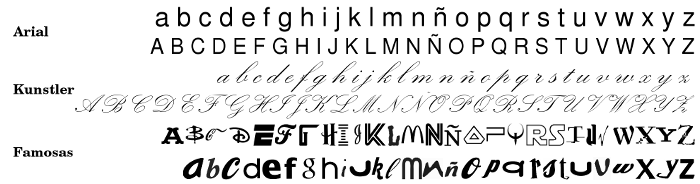
\includegraphics[scale=0.35]{graficos/letras.png}
      \caption{Conjunto completo de letras utilizadas en el experimento}
      \label{figura:conjuntoLetras}
    \end{figure}
\end{frame}



\section{Results}
\begin{frame}
  \frametitle{Results}
    \begin{table}
	\tiny
	\centering
	\label{tabla:cantidadBurbujas}
	\caption{Cantidad de burbujas promedio necesarias para la identificación de las letras}
	\begin{tabular}{c|r|r|r|c|r|r|r}
	    \hline
	    \multirow{2}{*}{\textbf{Letra}} & \multicolumn{3}{|c|}{\textbf{Tipografía}} & \multirow{2}{*}{\textbf{Letra}} & \multicolumn{3}{|c}{\textbf{Tipografía}} \\
	    \cline{2-4}\cline{6-8}
		& \textbf{Arial} & \textbf{Kunstler} & \textbf{Famosas} &     & \textbf{Arial} & \textbf{Kunstler} & \textbf{Famosas} \\\hline\hline
	    \textbf{A}   & 14   &   35   &   16   &   \textbf{a}   & 14   &   28   &   20   \\\hline
	    \textbf{B}   & 14   &   35   &   22   &   \textbf{b}   & 18   &   37   &   24   \\\hline
	    \textbf{C}   & 12   &   26   &   26   &   \textbf{c}   & 14   &   30   &   22   \\\hline
	    \textbf{D}   & 14   &   31   &   22   &   \textbf{d}   & 18   &   31   &   16   \\\hline
	    \textbf{E}   & 16   &   31   &   20   &   \textbf{e}   & 20   &   37   &   18   \\\hline
	    \textbf{F}   & 22   &   31   &   18   &   \textbf{f}   & 20   &   37   &   22   \\\hline
	    \textbf{G}   & 16   &   26   &   30   &   \textbf{g}   & 16   &   28   &   18   \\\hline
	    \textbf{H}   & 20   &   31   &   22   &   \textbf{h}   & 18   &   30   &   18   \\\hline
	    \textbf{I}   & 18   &   39   &   24   &   \textbf{i}   & 20   &   30   &   24   \\\hline
	    \textbf{J}   & 16   &   41   &   24   &   \textbf{j}   & 22   &   26   &   24   \\\hline
	    \textbf{K}   & 12   &   30   &   16   &   \textbf{k}   & 14   &   33   &   22   \\\hline
	    \textbf{L}   & 16   &   31   &   26   &   \textbf{l}   & 26   &   30   &   20   \\\hline
	    \textbf{M}   & 14   &   39   &   14   &   \textbf{m}   & 16   &   28   &   16   \\\hline
	    \textbf{N}   & 16   &   39   &   18   &   \textbf{n}   & 20   &   26   &   22   \\\hline
	    \textbf{Ñ}   & 18   &   39   &   12   &   \textbf{ñ}   & 20   &   26   &   22   \\\hline
	    \textbf{O}   & 16   &   30   &   22   &   \textbf{o}   & 16   &   33   &   22   \\\hline
	    \textbf{P}   & 14   &   33   &   22   &   \textbf{p}   & 16   &   30   &   22   \\\hline
	    \textbf{Q}   & 18   &   35   &   18   &   \textbf{q}   & 24   &   37   &   20   \\\hline
	    \textbf{R}   & 12   &   28   &   14   &   \textbf{r}   & 26   &   33   &   26   \\\hline
	    \textbf{S}   & 12   &   35   &   16   &   \textbf{s}   & 14   &   28   &   22   \\\hline
	    \textbf{T}   & 18   &   33   &   20   &   \textbf{t}   & 20   &   28   &   18   \\\hline
	    \textbf{U}   & 16   &   26   &   28   &   \textbf{u}   & 18   &   26   &   16   \\\hline
	    \textbf{V}   & 12   &   33   &   30   &   \textbf{v}   & 20   &   37   &   22   \\\hline
	    \textbf{W}   & 16   &   37   &   18   &   \textbf{w}   & 14   &   33   &   22   \\\hline
	    \textbf{X}   & 10   &   31   &   14   &   \textbf{x}   & 10   &   26   &   10   \\\hline
	    \textbf{Y}   & 14   &   28   &   14   &   \textbf{y}   & 16   &   24   &   14   \\\hline
	    \textbf{Z}   & 12   &   28   &   18   &   \textbf{z}   & 12   &   28   &   12   \\\hline
	\end{tabular}
    \end{table}
\end{frame}


\section{Resumen}
\begin{frame}
  \frametitle{Resumen}
  \begin{itemize}
    \item \pause Para obtener Síntesis de Habla expresiva se debe tener en cuenta la situación de diálogo completa \pause
    \begin{itemize}
      \item Intenciones \pause
      \item Características de hablante/oyente \pause
      \item Relación con el oyente \pause
      \item Progreso del diálogo y nivel de entendimiento \pause
    \end{itemize}
    \item Cada técnica tiene distintas opciones para controlar la expresividad \pause
    \item Se debe regular la naturalidad obtenida vs. el control sobre lo sintetizado \pause
    \item La síntesis basada en HMM puede mejorar las limitaciones de la Selección de Unidades (datos, flexibilidad) \pause
    \item La incorporación de expresiones y contenido no-verbal puede sumar a la expresividad, pero no debe utilizarse en exceso \pause
    \item El aprendizaje automático de reglas presenta una oportunidad (e.g. para sínt. por formantes, articulación)
  \end{itemize}
\end{frame}


\end{document}
